% !TeX encoding = UTF-8

\chapter{ANÁLISE DOS RESULTADOS}\label{ch:resultados}

Este capítulo tem como finalidade apresentar os resultados obtidos através das implementações demonstrados no \autoref{ch:implementacao}.

\section{APRESENTAÇÃO DOS RESULTADOS}

Após o mapeamento das informações do \textit{DataFrame},  ... conjunto de dados coletados, \autoref{lingua}.

\begin{grafico}[h]
	\centering
	\fbox{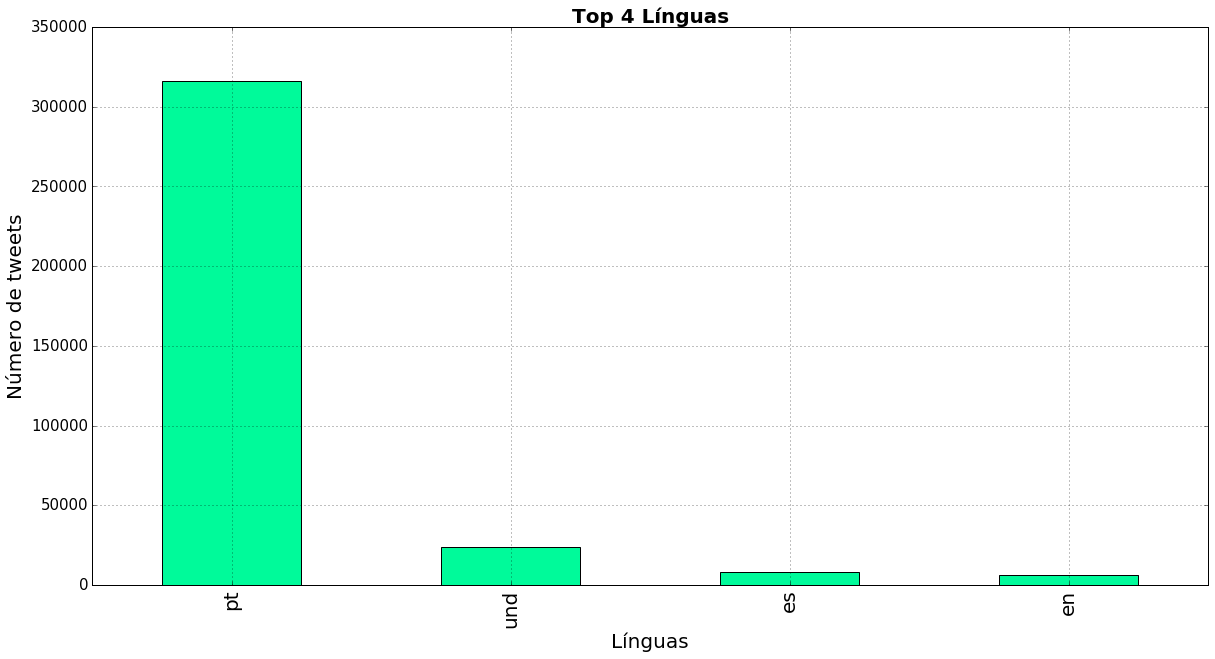
\includegraphics[width=1\textwidth]{linguas}}
	\caption{Idiomas que mais realizaram \textit{tweets}}
	\fonte{Elaborado pelo autor}
	\label{lingua}
\end{grafico}

\begin{table}[h]
\centering
\caption{Um nome qualquer}
\vspace{0.5cm}
\begin{tabular}{r|l|r}

Posição & País & IDH \\ % Note a separação de col. e a quebra de linhas
\hline                               % para uma linha horizontal
1 & Noruega        & .955 \\
2 & Austr{\'a}lia  & .938 \\
3 & EUA            & .937 \\
4 & Holanda        & .921 \\
5 & Alemanha       & .920            % não é preciso quebrar a última linha

\end{tabular}
\end{table}









